\usetikzlibrary{shapes.geometric, arrows, overlay-beamer-styles}

\tikzstyle{picnode} = [rectangle, minimum size=0.45\textwidth, draw=black]
\tikzstyle{textnode} = [rectangle, rounded corners, text centered, draw=black]

\begin{tikzpicture}[node distance=4cm]

\node (input) [textnode] {
  \tiny
  HCP Assessments
};

\node (cdss) [picnode, right of=input] {
  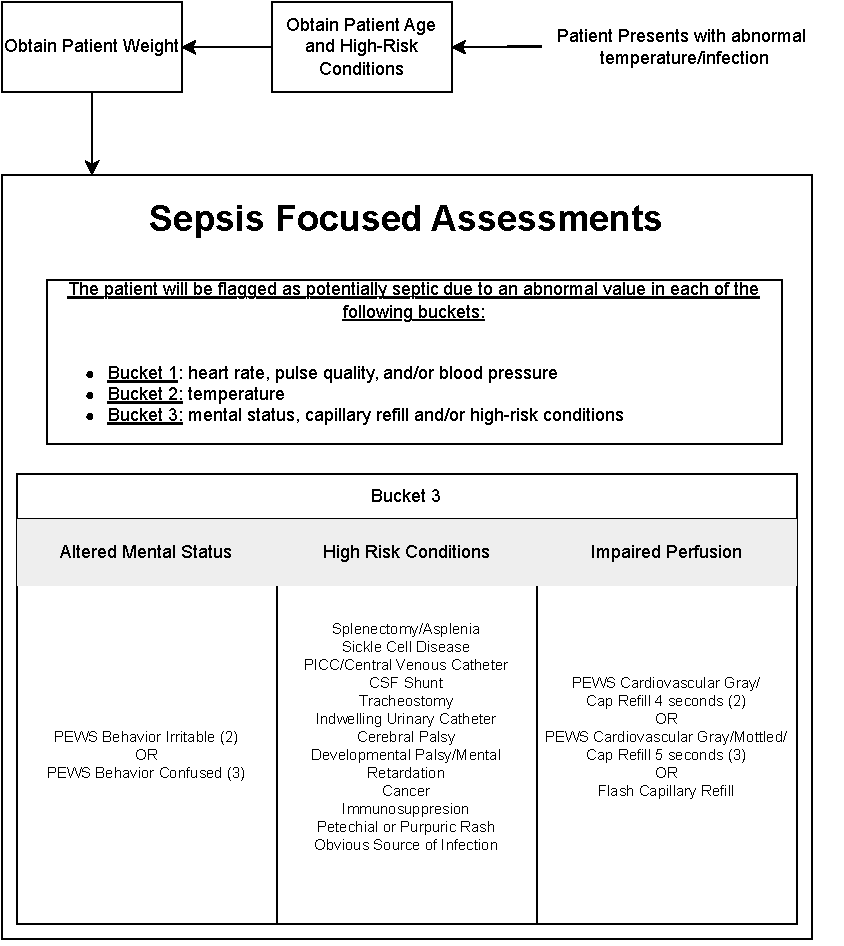
\includegraphics[width=0.4\textwidth]{sepsis-screening-osf}
};

\node (sensor) [textnode, below of=cdss] {
  \tiny
  Sensors + Electronic Health Records
};
\draw<2-> node (advice) [textnode, right of=cdss, fill=red!30] {
  \tiny
  Decision Support
};
\path[->]
  (sensor) edge  (cdss)
  (input) edge (cdss)
  ;

\draw<2-> (cdss) edge[->] (advice);

\end{tikzpicture}
